% This work is made available under the terms of the
% Creative Commons Attribution-ShareAlike 4.0 license,
% http://creativecommons.org/licenses/by-sa/4.0/.

\documentclass[a4paper]{book}

\usepackage{wrapfig}
\usepackage{graphicx}
\usepackage{hyperref}
\usepackage{multirow}
\usepackage{scalefnt}
\usepackage{tikz}

% watermark -- for draft stage
%\usepackage[firstpage]{draftwatermark}
%\SetWatermarkLightness{0.9}
%\SetWatermarkScale{5}

% Copyright (c) 2009 by the University of Waikato, Hamilton, NZ. 
% This work is made available under the terms of the 
% Creative Commons Attribution-ShareAlike 3.0 license, 
% http://creativecommons.org/licenses/by-sa/3.0/. 
%
% Version: $Revision$

\newenvironment{tight_itemize}{
\begin{itemize}
  \setlength{\itemsep}{1pt}
  \setlength{\parskip}{0pt}
  \setlength{\parsep}{0pt}}{\end{itemize}
}

\newenvironment{tight_enumerate}{
\begin{enumerate}
  \setlength{\itemsep}{1pt}
  \setlength{\parskip}{0pt}
  \setlength{\parsep}{0pt}}{\end{enumerate}
}

% if you just need a simple heading
% Usage:
%   \heading{the text of the heading}
\newcommand{\heading}[1]{
  \vspace{0.3cm} \noindent \textbf{#1} \newline
}

\newcommand{\icon}[1]{\tikz[baseline=-3pt]\node[inner sep=0pt,outer sep=0pt]{\includegraphics[height=1.1em]{#1}};}


\title{
  \textbf{ADAMS} \\
  {\Large \textbf{A}dvanced \textbf{D}ata mining \textbf{A}nd \textbf{M}achine
  learning \textbf{S}ystem} \\
  {\Large Module: adams-xml} \\
  \vspace{1cm}
  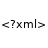
\includegraphics[width=2cm]{images/xml-module.png} \\
}
\author{
  Peter Reutemann
}

\setcounter{secnumdepth}{3}
\setcounter{tocdepth}{3}

\begin{document}

\begin{titlepage}
\maketitle

\thispagestyle{empty}
\center
\begin{table}[b]
	\begin{tabular}{c l l}
		\parbox[c][2cm]{2cm}{\copyright 2019} &
		\parbox[c][2cm]{5cm}{
\includegraphics[width=5cm]{images/coat_of_arms.pdf}} \\
	\end{tabular}
	
\includegraphics[width=12cm]{images/cc.png} \\
\end{table}

\end{titlepage}

\tableofcontents
%\listoffigures
%\listoftables

%%%%%%%%%%%%%%%%%%%%%%%%%%%%%%%%%%%
\chapter{Flow}
ADAMS offers some basic handling for XML\cite{xml}, XSLT\cite{xslt} and XPath\cite{xpath}.
The following sources are available:
\begin{tight_itemize}
	\item \textit{NewDOMDocument} -- creates an empty DOM document.
\end{tight_itemize}
The following transformers are available:
\begin{tight_itemize}
	\item \textit{AddDOMAttribute} -- adds an attribute and its value to the
	node passing through.
	\item \textit{AddDOMNode} -- appends a child new to the node passing through.
	\item \textit{XMLFileReader} -- reads the specific XML file and forwards
	a DOM document.
	\item \textit{XPath} -- applies an XPath expression to the incoming DOM document.
	\item \textit{XSLT} -- applies an XSLT stylesheet to the incoming DOM document.
\end{tight_itemize}
The following sinks are available:
\begin{tight_itemize}
	\item \textit{DOMDisplay} -- simple tree view of a DOM node.
	\item \textit{XMLFileWriter} -- writes the DOM document to disk.
\end{tight_itemize}
The following conversions are available:
\begin{tight_itemize}
	\item \textit{DOMToString} -- turns the DOM object into an XML string.
	\item \textit{DOMToProperties} -- flattens the DOM object into a Java
	Properties object (key-value pairs).
	\item \textit{DOMNodeToString} -- turns the DOM node into an XML string.
	\item \textit{DOMNodeListToArray} -- turns the list of DOM nodes into an array.
	\item \textit{PrettyPrintXML} -- turns an XML string into a pretty-printed XML string.
	\item \textit{XMLToDOM} -- parses the XML string and generates a DOM
	object.
\end{tight_itemize}

%%%%%%%%%%%%%%%%%%%%%%%%%%%%%%%%%%%
\chapter{Tools}

\section{Pretty print XML}
In order to preserve space, XML is often optimized and removes any unnecessary
whitespaces. However, for a human to inspect such data, it is much more useful
to have it properly indented, aka \textit{pretty printed}. Figure \ref{pretty_print_xml}
shows a screenshot of the \textit{Pretty print XML} tool that allows you to
turn XML into a more human-readable format.
\begin{figure}[htb]
  \centering
  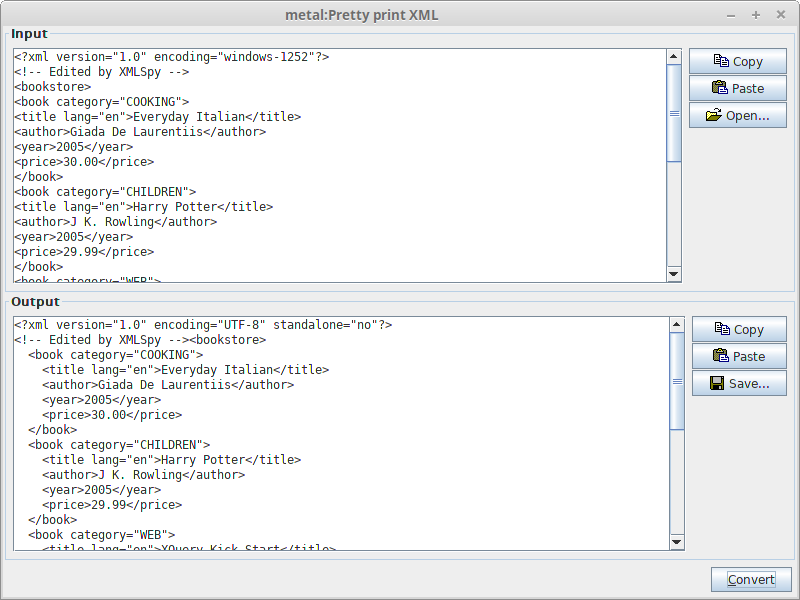
\includegraphics[width=12.0cm]{images/pretty_print_xml.png}
  \caption{Pretty print XML}
  \label{pretty_print_xml}
\end{figure}

%%%%%%%%%%%%%%%%%%%%%%%%%%%%%%%%%%%
% Copyright (c) 2009-2012 by the University of Waikato, Hamilton, NZ. 
% This work is made available under the terms of the 
% Creative Commons Attribution-ShareAlike 4.0 license,
% http://creativecommons.org/licenses/by-sa/4.0/.
%
% Version: $Revision$

\begin{thebibliography}{999}
	% to make the bibliography appear in the TOC
	\addcontentsline{toc}{chapter}{Bibliography}

    % references
	\bibitem{adams}
		\textit{ADAMS} -- Advanced Data mining and Machine learning System \\
		\url{https://adams.cms.waikato.ac.nz/}{}

	\bibitem{esrigrid}
	 	\textit{Esri Grid} -- a raster GIS file format deveoped by Esri. \\
		\url{https://en.wikipedia.org/wiki/Esri\_grid}{}

	\bibitem{kml}
	 	\textit{Keyhole Markup Language} -- an XML notation for expressing
	 	geographic annotation and visualization within Internet-based,
	 	two-dimensional maps and three-dimensional Earth browsers. \\
		\url{http://en.wikipedia.org/wiki/Keyhole\_Markup\_Language}{}

	\bibitem{postgresql}
	 	\textit{PostgreSQL} -- a powerful, open source object-relational
	 	database system. \\
		\url{http://www.postgresql.org/}{}

	\bibitem{postgis}
		\textit{PostGIS} -- a spatial database extender for PostgreSQL
		object-relational database. It adds support for geographic
		objects allowing location queries to be run in SQL.  \\
		\url{http://postgis.net/}{}

	\bibitem{srid4269}
	 	\textit{SRID 4269} -- or NAD 83 (North American Datum). \\
		\url{http://spatialreference.org/ref/epsg/4269/}{}

	\bibitem{mysql}
		\textit{MySQL} -- an open-source relational database management
		system (RDBMS) \\
		\url{http://www.mysql.com/}{}

\end{thebibliography}


\end{document}
